
% case name
\chapter{Bergenmeersen test case}
%
%
% - Purpose & Description:
%     These first two parts give reader short details about the test case,
%     the physical phenomena involved, the geometry and specify how the numerical solution will be validated
\section{Purpose}
%
The purpose of this test-case is to test the culvert functionality in TELEMAC-3D with a quantitative comparison to
measurements of the flow rates through the culverts and the water levels on each side of the culverts.

\section{Description}
%
% - Physical parameters:
%     This part specifies details all the physical parameters
%\subsection{Physical parameters}
A recent (2013) example of the implementation of a Flood Control Area (FCA) with a controlled reduced 
tide (CRT) system is located in Bergenmeersen. 
The ring dike that surrounds the FCA has a crest level of 8 m TAW
(Tweede Algemene Waterpassing, the reference level in Belgium;
0 m TAW corresponds to the average sea level at low water in Ostende port)
and the overflow dike has a crest level of 6.8 m TAW.
The configuration used for the inlet and outlet culverts is shown in the Figure \ref{fig:bergenmeersen_figure1}.
Three outlet culverts were built to add to other older three outlet culverts that existed in the area. 
Above the new outlet culverts, six new inlet culverts were built and at their entrance weirs (i.e. wooden beams) 
with different heights were added (Figure \ref{fig:bergenmeersen_figure1} and Figure \ref{fig:bergenmeersen_figure2}). 
At each inlet and outlet culvert the flow is separated into two parts at the entrance of the culvert 
by a kind of pilar and then converges again right after this pilar. 
Figure \ref{fig:bergenmeersen_figure3} shows an example of the trash screens that are present. 
Table \ref{tab:bergenmeersen_table1} gives an overview of the characteristics of these new inlet and outlet culverts.

To test the new culvert functionality implemented in TELEMAC-3D this new configuration of in- and outlet culverts is tested. 
The quality of the results can be assessed compared to measurements of the mean water levels inside the flood control area, 
outlet discharges, inlet discharges and mean water levels in the river side. 

\begin{figure}[H]
\begin{center}
  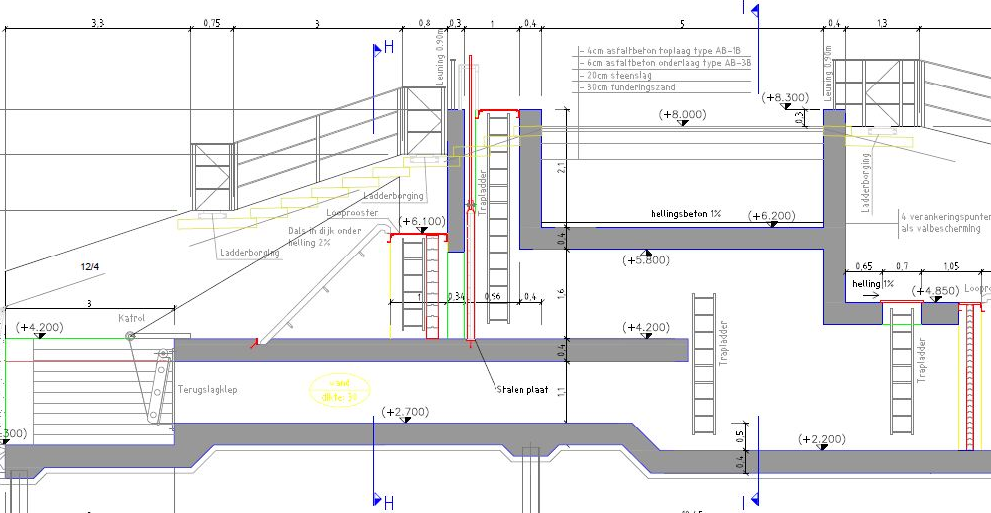
\includegraphics[scale=0.5]{figure1.png}
\end{center}
\caption{Bergenmeersen test case: detail of the side view of 
the construction of the new inlet and outlet culverts in Bergenmeersen.}
\label{fig:bergenmeersen_figure1}
\end{figure}

\begin{figure}[H]
\begin{center}
  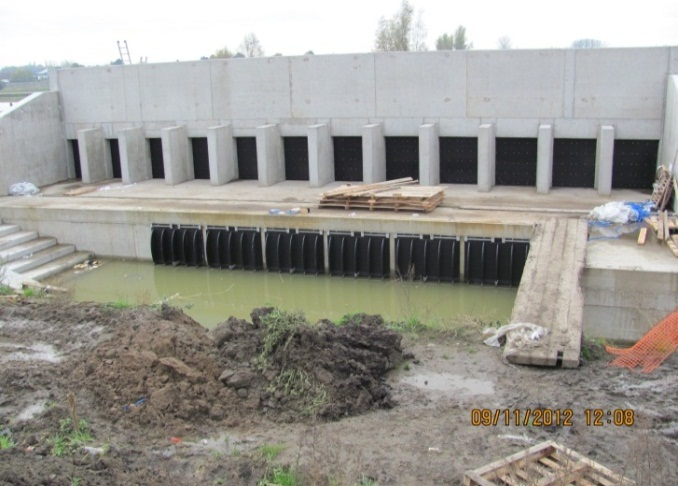
\includegraphics[scale=1.0]{figure2.png}
\end{center}
\caption{Bergenmeersen test case: inlet and outlet culvert configuration on the river side (construction phase) (Patrimoniumdatabank W\&Z).}
\label{fig:bergenmeersen_figure2}
\end{figure}

\begin{figure}[H]
\begin{center}
  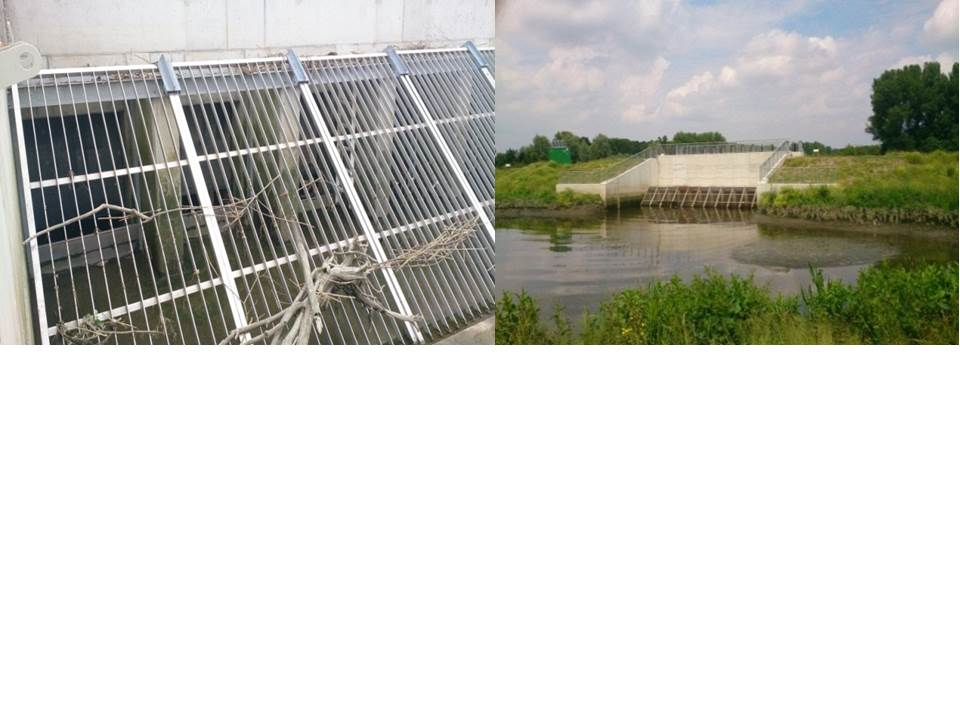
\includegraphics[scale=0.5, trim = 0 300 0 0, clip]{figure3.png}
\end{center}
\caption{Bergenmeersen test case: View on the inlet culverts from the river side and inlet and outlet culverts from the FCA side.}
\label{fig:bergenmeersen_figure3}
\end{figure}

\begin{table}[H]
\caption{Characteristics of the new inlet and outlet culverts of the new 
FCA/CRT in Bergenmeersen.}\label{tab:bergenmeersen_table1}
\begin{center}\begin{tabular}{|c|c|c|c|c|}
\hline
~ & \textbf{Inlet} & \textbf{Inlet} & \textbf{Outlet} & \textbf{Outlet}\\
~ & \textbf{(Scheldt side)} & \textbf{(FCA side)} & \textbf{(Scheldt side)} & \textbf{(FCA side)}\\
\hline
\textbf{Number of culverts} & \multicolumn{2}{c|}{6} & \multicolumn{2}{c|}{3} \\
\hline
\textbf{Culvert width (m)} & \multicolumn{2}{c|}{2.7} & \multicolumn{2}{c|}{3} \\
\hline
\textbf{Culvert length (m)} & \multicolumn{2}{c|}{9.5} & \multicolumn{2}{c|}{18} \\
\hline
\textbf{Culvert height (m)} & 1.6 & 2.25 & 1.1 & 2.25\\
\hline
\textbf{Level of culvert floor} & 4.2 & 2.2 & 2.7 & 2.2\\
\textbf{(m TAW)} & ~ & ~ & ~ & ~\\
\hline
\textbf{Crest level of weirs} & 4.2/4.2/4.2/ & ~ & ~ & ~ \\
\textbf{(m TAW)} & 4.35/4.5/4.5 & ~ & ~ & ~ \\
\hline
\end{tabular}\end{center}
\end{table}
%
% Experimental results (if needed)
\subsection{Measurements}
The quality of the numerical results can be assessed compared to measurements of the mean water levels inside the flood control area, 
outlet discharges, inlet discharges and mean water levels in the river side. 
Measurements were perfomed by Flanders Hydraulic Research in Bergenmeersen 
within a 13 hour campaign during the 10th September, 2013. 
They obtained water levels in front of the culverts in the Scheldt 
and in the floodplain sides and discharges for the inlet and outlet culverts. 
The model results for this period will be compared with the measurements. 
%
% bibliography can be here or at the end
%\subsection{Reference}
%
% Section for computational options
\section{Computational options}
%
% - Mesh:
%     This part describes the mesh used in the computation
\subsection{Mesh}
The mesh of the computational domain is shown in Figure \ref{fig:bergenmeersen_figure4}.
The mesh is cut out of an early version of the Scaldis model. 
It has a resolution of about 8 m in the river side, and 10 m in the floodplain. 
Five horizontal layers are uniformly imposed in the model. 
Detailed bathymetric/topographic data from 2013 is available and used for this model.
\begin{figure}[H]
\begin{center}
  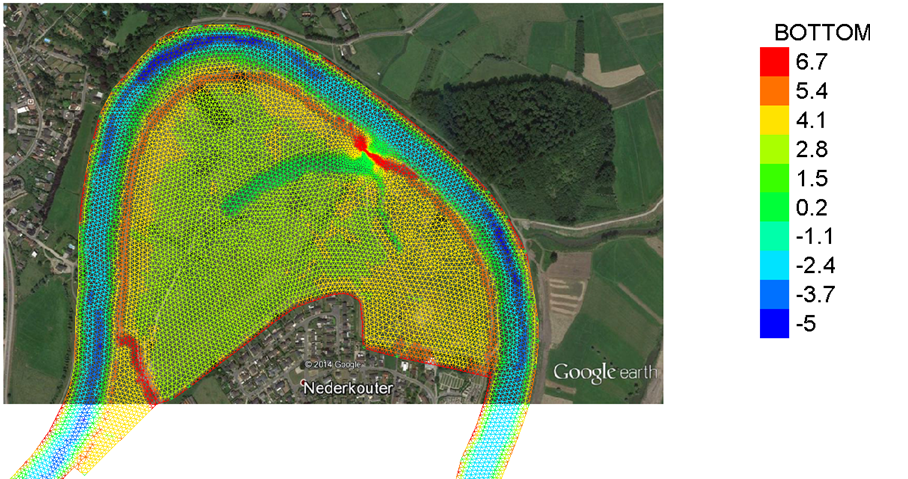
\includegraphics[scale=0.5]{figure4.png}
\end{center}
\caption{Planview of the computational domain to model the FCA/CRT in Bergenmeersen.
The colour scale represents de bottom values (m TAW).}
\label{fig:bergenmeersen_figure4}
\end{figure}
%
% - Initial and boundary conditions:
%     This part details both initial and boundary conditions used to simulate the case
\subsection{Initial and boundary conditions}
The water levels in the Scheldt river are obtained at the Wetteren tidal station. 
These values are used as the downstream boundary condition for the hydrodynamic model. 
Upstream a discharge boundary condition is imposed.
%
% - Numerical parameters:
%     This part is used to specify the numerical parameters used
%     (adaptive time step, mass-lumping when necessary...)
\subsection{Numerical parameters}
The simulation time is about one day (10th September 2014) corresponding to the time period 
for which measurements of mean water levels were available. 
The time step is set to 5 seconds, providing, together with the chosen mesh resolution, a stable simulation.

The bottom friction is taken into account in the model through the Manning Strickler’s parameter $n$, set to $0.02 s.m^{-1/3}$. 
The horizontal and vertical turbulence viscosity coefficients are both set to $0.01 m^2s^{-1}$.

\subsection{Culvert parameters}
Table \ref{tab:bergenmeersen_table2} shows the file that the user has to give to TELEMAC-3D in order to take 
into account the culverts for this FCA with CRT in the Bergenmeersen test case. 
Besides this new structure there were already in the area three outlet sluices 
also represented in the input text file as outlet 3 to outlet 6 
(information for these outlet sluices is obtained from the Patrimoniumdatabank W\&Z)
Once again the different head loss coefficients are used to calibrate the model 
with the experimental data. 
Most of the parameters are maintained comparatively with the Lippenbroek test case. 
But there are some exceptions, given the fact that the inlet and outlet culvert configurations are also different. 
For instance the head loss coefficients at the entrance of the inlet are increased in order to take 
into account the effect of the flow being split into two parts by a pillar. 
Following the expression given by Carlier (1972), the head loss due to the presence of pillars is about Cp $\approx 0.4$ 
and therefore CE1 becomes CE1=C1+Cp. 
There is also at the exit of the outlet sluices the separation of the flow into two parts. 
This effect is taken into account in the head loss due to a valve, increasing the value for CV. 
Also during the measurement campaign, the trash screens at the inlet sluices are 
not cleaned and therefore this coefficient is increased both for the inlet and outlet sluices.

\begin{table}[H]
\caption{Input data for the culvert subroutine in TELEMAC-3D to model the Bergenmeersen FCA/CRT.}\label{tab:bergenmeersen_table2}
\small
\begin{center}\begin{tabular}{|c|c|c|c|c|c|c|c|c|c|c|c|c|c|c|c|}
\hline
~ & \textbf{CE1} & \textbf{CE2} & \textbf{CS1} & \textbf{CS2} & \textbf{CV} & \textbf{CT} & \textbf{C56} & \textbf{C5} & \textbf{CV5} & \textbf{W} & \textbf{D1} & \textbf{D2} & \textbf{N} & \textbf{L} & \textbf{CP}\\
\hline
\textbf{Inlet 1} & 0.9 & 0.5 & 1 & 1 & 0 & 1 & 10 & 6 & 0 & 2.7 & 1.45 & 2.25 & 0.015 & 9.5 & 0 \\
\hline
\textbf{Inlet 2} & 0.9 & 0.5 & 1 & 1 & 0 & 1 & 10 & 6 & 0 & 2.7 & 1.6 & 2.25 & 0.015 & 9.5 & 0 \\
\hline
\textbf{Inlet 3} & 0.9 & 0.5 & 1 & 1 & 0 & 1 & 10 & 6 & 0 & 2.7 & 1.6 & 2.25 & 0.015 & 9.5 & 0 \\
\hline
\textbf{Inlet 4} & 0.9 & 0.5 & 1 & 1 & 0 & 1 & 10 & 6 & 0 & 2.7 & 1.6 & 2.25 & 0.015 & 9.5 & 0 \\
\hline
\textbf{Inlet 5} & 0.9 & 0.5 & 1 & 1 & 0 & 1 & 10 & 6 & 0 & 2.7 & 1.6 & 2.25 & 0.015 & 9.5 & 0 \\
\hline
\textbf{Inlet 6} & 0.9 & 0.5 & 1 & 1 & 0 & 1 & 10 & 6 & 0 & 2.7 & 1.6 & 2.25 & 0.015 & 9.5 & 0 \\
\hline
\textbf{Outlet 1} & 0.5 & 0.5 & 1 & 1 & 12 & 1 & 10 & 6 & 1.5 & 3 & 1.1 & 2.25 & 0.015 & 18.5 & 2 \\
\hline
\textbf{Outlet 2} & 0.5 & 0.5 & 1 & 1 & 12 & 1 & 10 & 6 & 1.5 & 3 & 1.1 & 2.25 & 0.015 & 18.5 & 2 \\
\hline
\textbf{Outlet 3} & 0.5 & 0.5 & 1 & 1 & 12 & 1 & 10 & 6 & 1.5 & 3 & 1.1 & 2.25 & 0.015 & 18.5 & 2 \\
\hline
\textbf{Outlet 4} & 0.5 & 0.5 & 1 & 1 & 12 & 1 & 10 & 6 & 1.5 & 1.5 & 1.8 & 2.55 & 0.015 & 20 & 2 \\
\hline
\textbf{Outlet 5} & 0.5 & 0.5 & 1 & 1 & 12 & 1 & 10 & 6 & 1.5 & 1.5 & 1.8 & 2.6 & 0.015 & 20 & 2 \\
\hline
\textbf{Outlet 6} & 0.5 & 0.5 & 1 & 1 & 12 & 1 & 10 & 6 & 1.5 & 1.5 & 1.8 & 2.55 & 0.015 & 20 & 2 \\
\hline
\end{tabular}\end{center}\normalsize
\end{table}
%
% - Results:
%     We comment in this part the numerical results against the reference ones,
%     giving understanding keys and making assumptions when necessary.
\section{Results}

Figure \ref{fig:bergenmeersen_figure5} shows the differences in water level in the 
river in front of the in- and outlet construction of Bergenmeersen. 
This figure shows that it is difficult to get the water levels in this model correct. 
The downstream water level boundary of this small model is not located at the same location 
as the Wetteren tidal measurement station, but more upstream.
Keeping this in mind Figure \ref{fig:bergenmeersen_figure6} shows the difference between measured 
and modeled water levels in the floodplain. 
The water level in the model follows a similar path as the measured water level. 
Given the complicated construction (in terms of translating this to an equation for discharge) 
of the in- and outlet structure, these results are a good approximation of reality.
In Figure \ref{fig:bergenmeersen_figure7} we see that the outlet discharge computed by the model fits 
fairly well the experimental data even if the numerical results overestimate the measurements around 12h. 
Regarding the inlet discharge, Figure \ref{fig:bergenmeersen_figure8} shows that the computed discharges are 
overestimated by the model, resulting on the overestimation seen in the mean water level in the FCA. 
A possible explanation for the discrepancies is that the inlet sluices have gates incorporated 
and in this test case it is considered that these gates are completely open. 
We have heard that in reality this is not the case and that the opening of these gates is 
changed several times over the last two years. 
The purpose of these gates is to close the area and prevent water from entering. 
There is no information on the openings of these gates at the time of this 13 hour measurement campaign.

\begin{figure}[H]
\begin{center}
  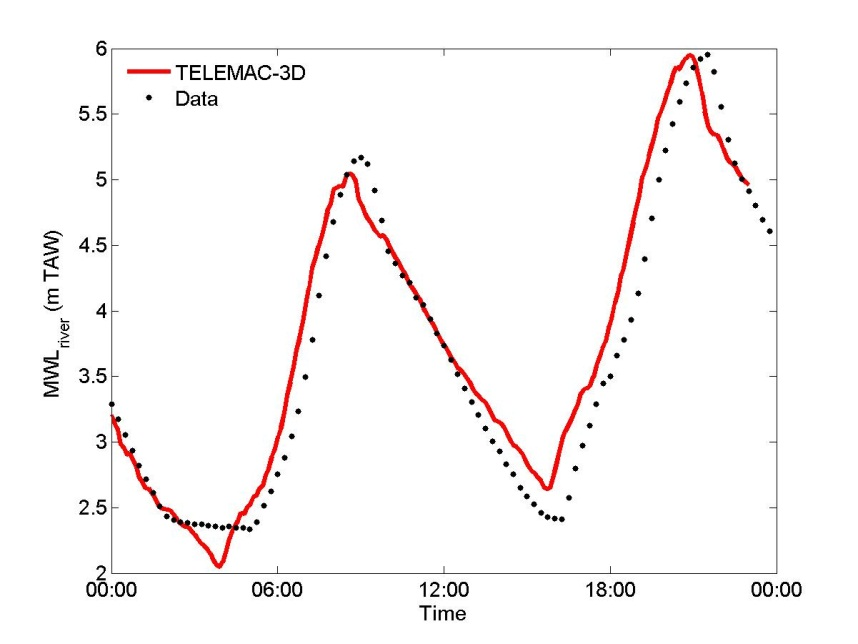
\includegraphics[scale=1]{figure5.png}
\end{center}
\caption{Bergenmeersen test case: comparison of the mean water level time evolution in the 
river between numerical results and measurements.}
\label{fig:bergenmeersen_figure5}
\end{figure}

\begin{figure}[H]
\begin{center}
  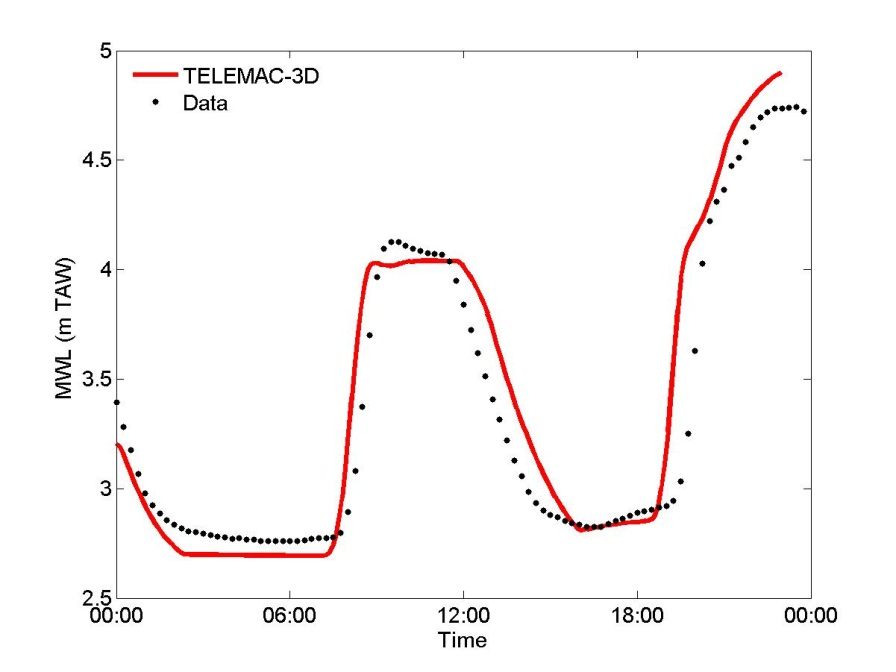
\includegraphics[scale=1]{figure6.png}
\end{center}
\caption{Bergenmeersen test case: comparison of the mean water level time 
evolution in the floodplain between numerical results and measurements.}
\label{fig:bergenmeersen_figure6}
\end{figure}

\begin{figure}[H]
\begin{center}
  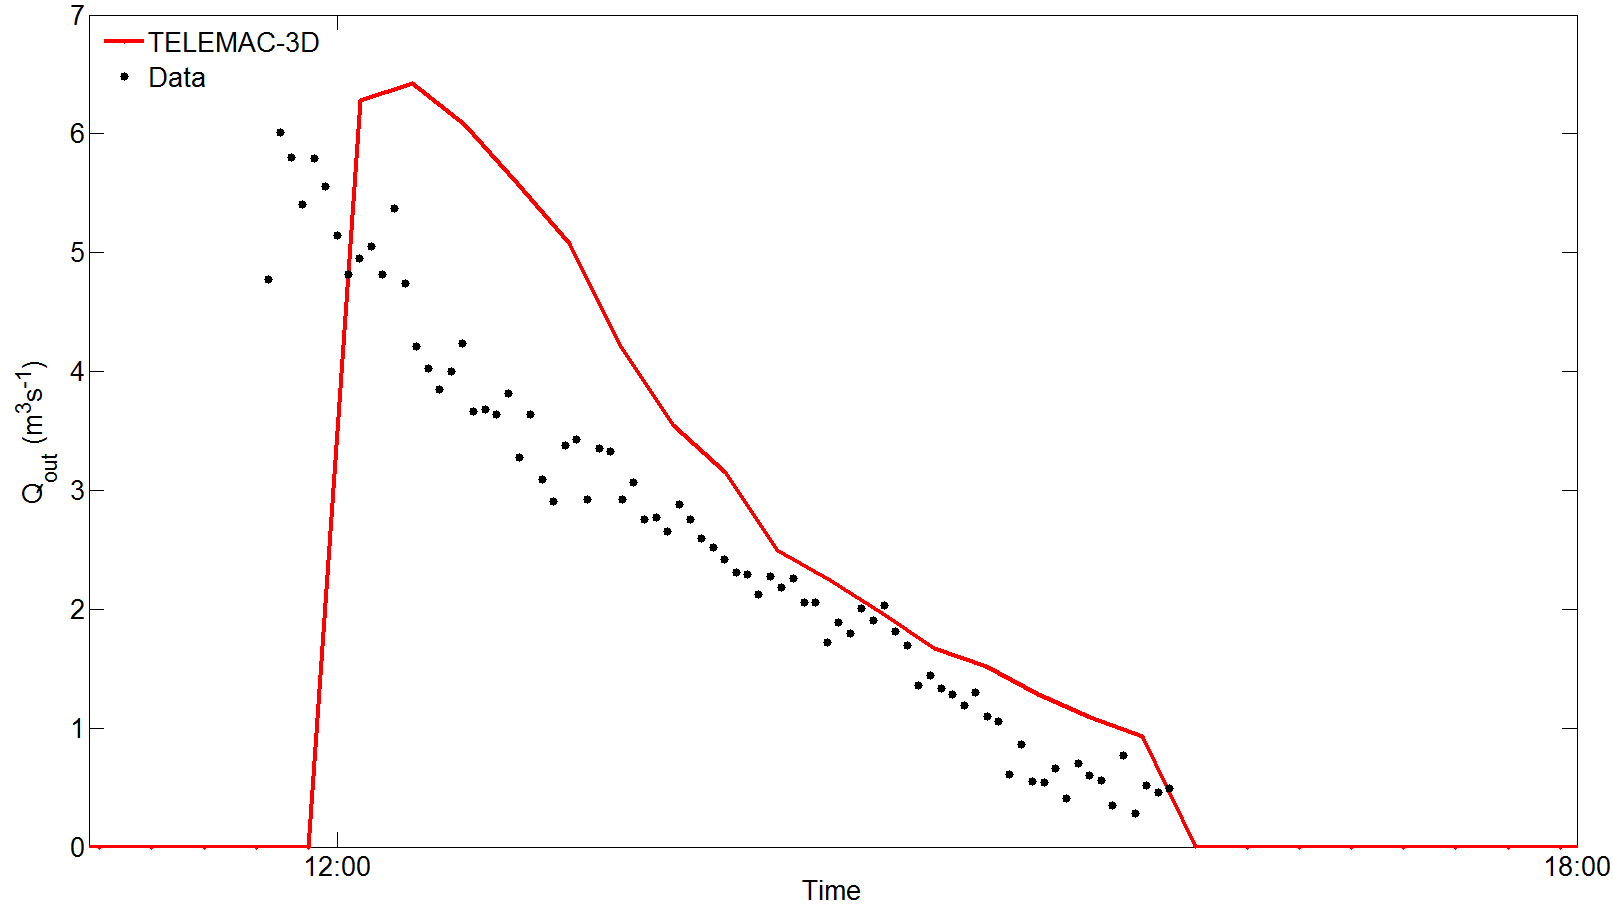
\includegraphics[scale=0.3]{figure7.png}
\end{center}
\caption{Bergenmeersen test case: comparison of outlet culvert discharges time evolution between numerical results and measurements.}
\label{fig:bergenmeersen_figure7}
\end{figure}
\begin{figure}[H]
\begin{center}
  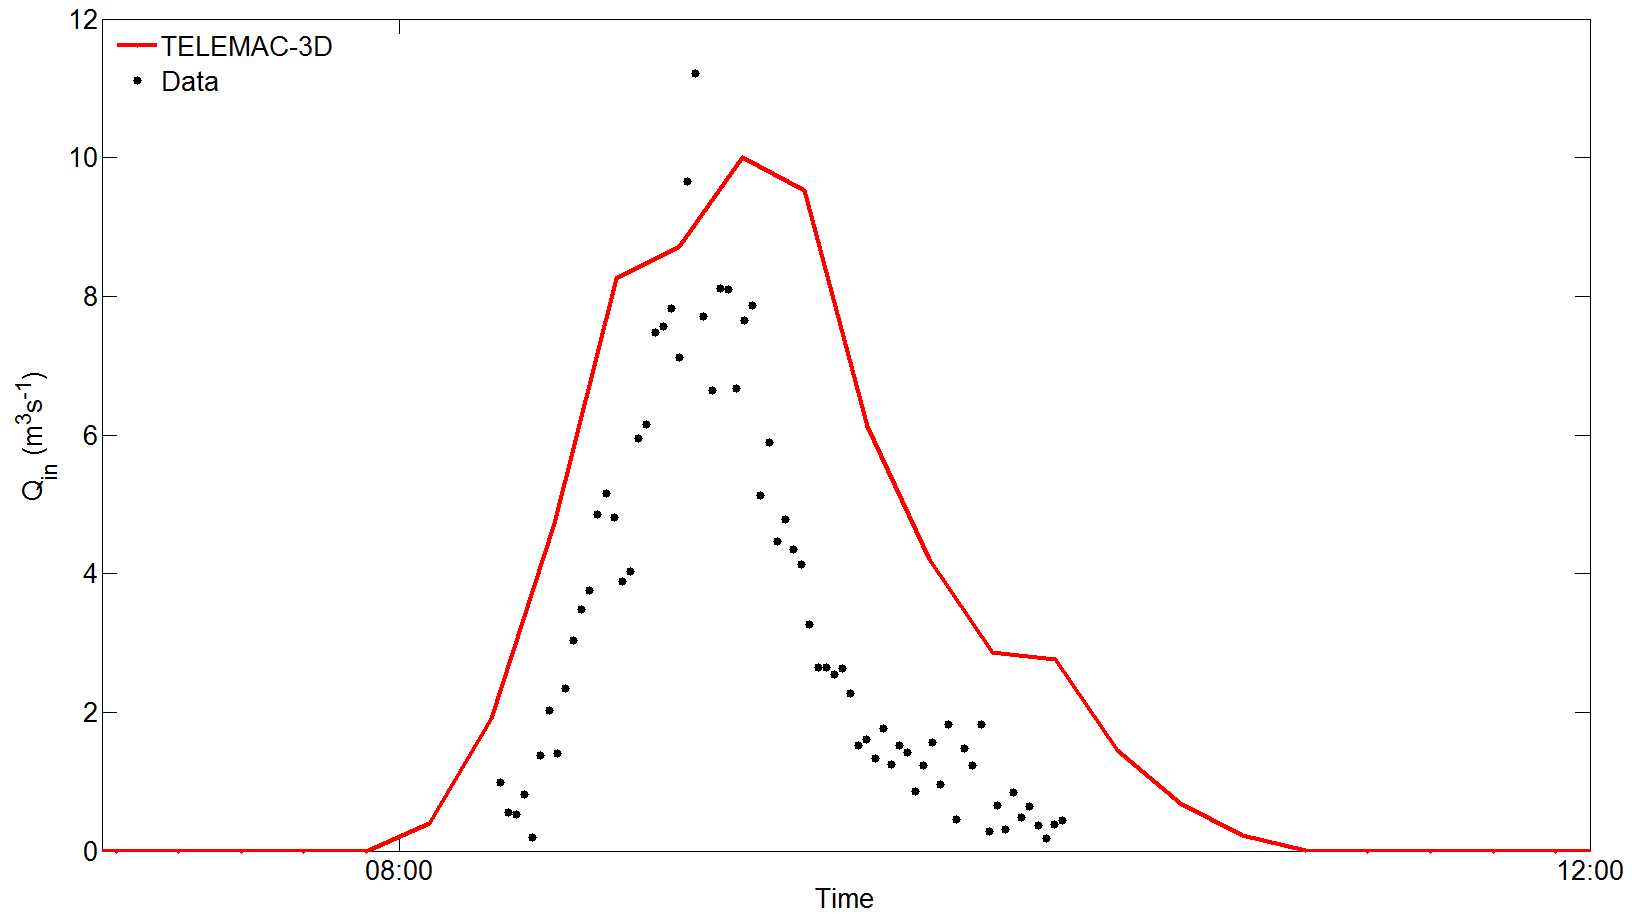
\includegraphics[scale=0.3]{figure8.png}
\end{center}
\caption{Bergenmeersen test case: comparison of inlet culvert discharges time evolution between numerical results and measurements.}
\label{fig:bergenmeersen_figure8}
\end{figure}

The normalized root mean square error is calculated for the mean water levels, outlet and inlet discharges (Table \ref{tab:bergenmeersen_table3}). 

\begin{table}[H]
\caption{Normalized root mean square error for the mean water level (MWL\_error), 
outlet discharge(Qout\_error) and inlet discharge (Qin\_error) 
in the Bergenmeersen test case.}\label{tab:bergenmeersen_table3}
\begin{center}\begin{tabular}{|c|c|}
\hline
\textbf{MWL\_error} & 0.275\\
\hline
\textbf{Qout\_error} & 0.453 \\
\hline
\textbf{Qin\_error} & 0.538 \\
\hline
\end{tabular}\end{center}
\end{table}

In Figure \ref{fig:bergenmeersen_figure9}, the flow types that predominate through the inlet and outlet culverts are presented. 
While for the former, flow types 2, 3 and 4 predominate, for the latter flow types 2 and 4 are the ones that occur the most.

\begin{figure}[H]
\begin{center}
  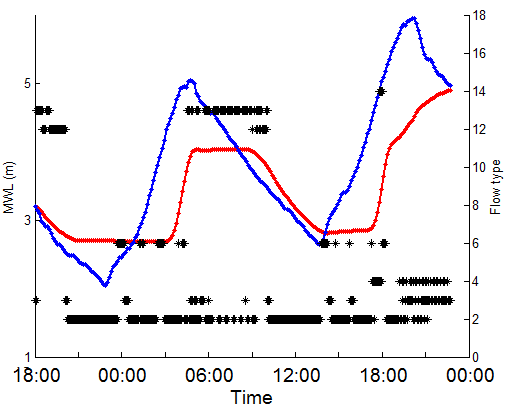
\includegraphics[scale=1]{figure9.png}
\end{center}
\caption{Bergenmeersen test case: mean water levels modelled by TELEMAC-3D in the river (blue line) 
and in the FCA (red line) and the corresponding flow types that occur during the time series. 
Flow through inlet culvert (type 2 - 6) and through outlet culvert (type 12 - 16)}
\label{fig:bergenmeersen_figure9}
\end{figure}

The results show that given some uncertainty like the representation of ditches and creeks in the topo-bathymetry of the model 
or the complexity of the in- and outlet structure, numerical results fit fairly well with data, 
both for the mean water levels and inlet and outlet discharges.

%
% bibliography
%\section{References}



